\documentclass[10pt]{beamer}

\usetheme{metropolis}

\usepackage{graphicx}
\usepackage{subcaption}
\usepackage{siunitx}
\usepackage{amsmath}
\usepackage{physics}
\usepackage{tikz-cd}
\usepackage[labelformat=empty]{caption}
\newtheorem{mydef}{Definition}
\newtheorem{thm}{Theorem}
\setbeamertemplate{itemize subitem}[square]

\title{New ``Symmetries'' of the Standard Model}
\author{Duncan Wilkie}
\date{2 December 2022}

\begin{document}

\begin{frame}
  \titlepage
\end{frame}

\begin{frame}
  % What the paper is
  \frametitle{Paper}
  \begin{center}
    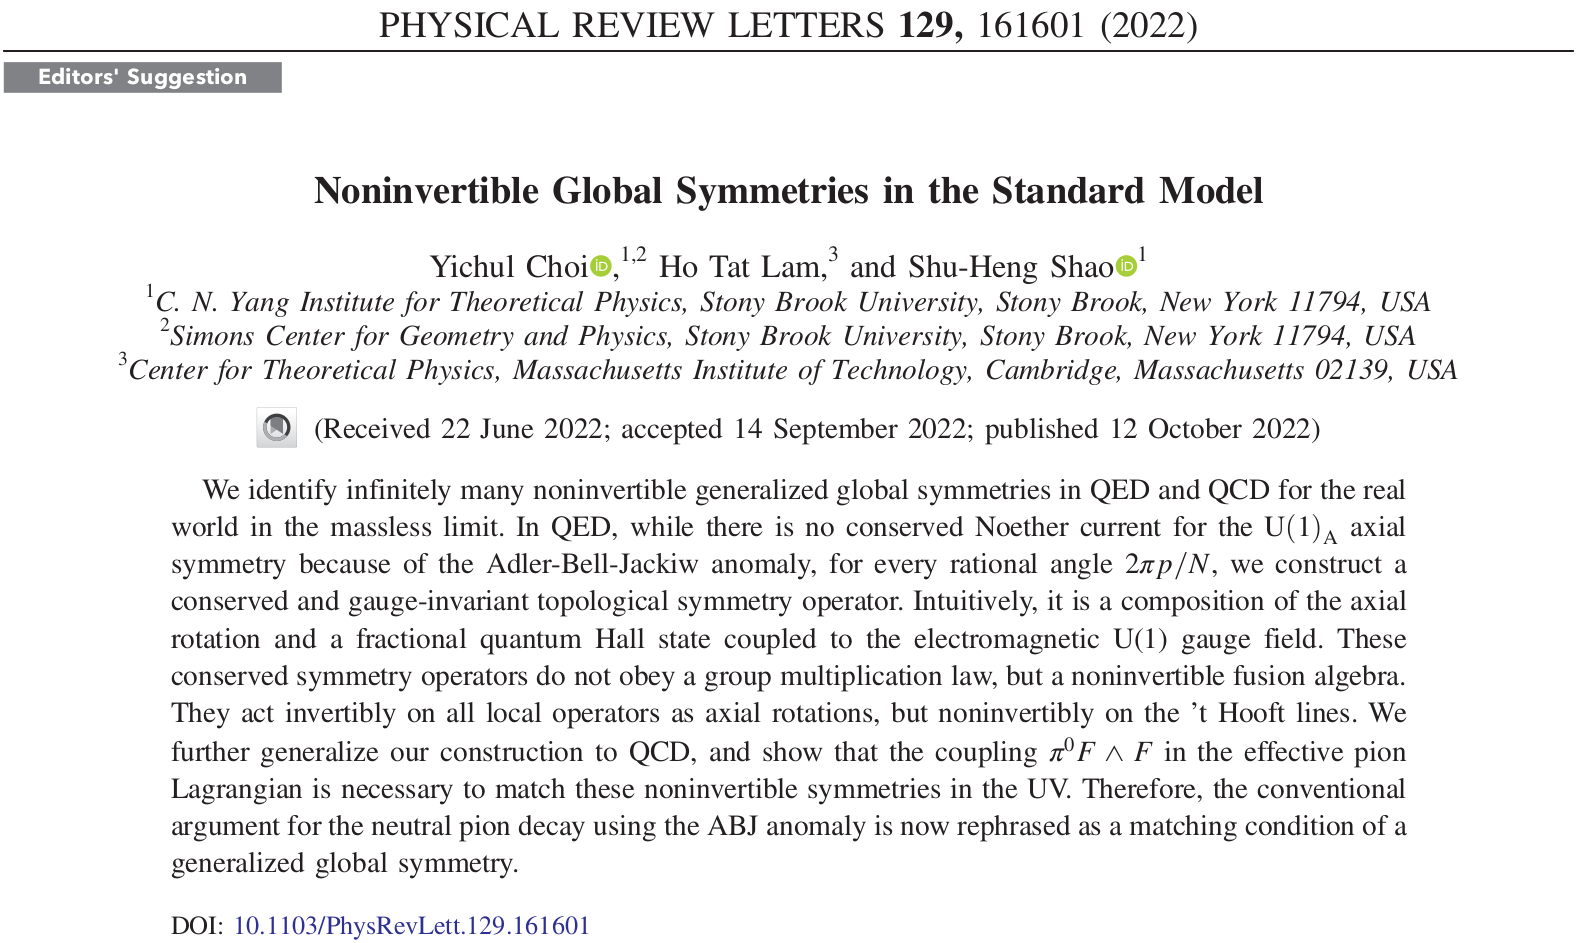
\includegraphics[scale=0.28]{abstract.png}
  \end{center}
\end{frame}

\begin{frame}
  % Terms requiring explanation
  \frametitle{Paper}
  \begin{figure}
    \centering
    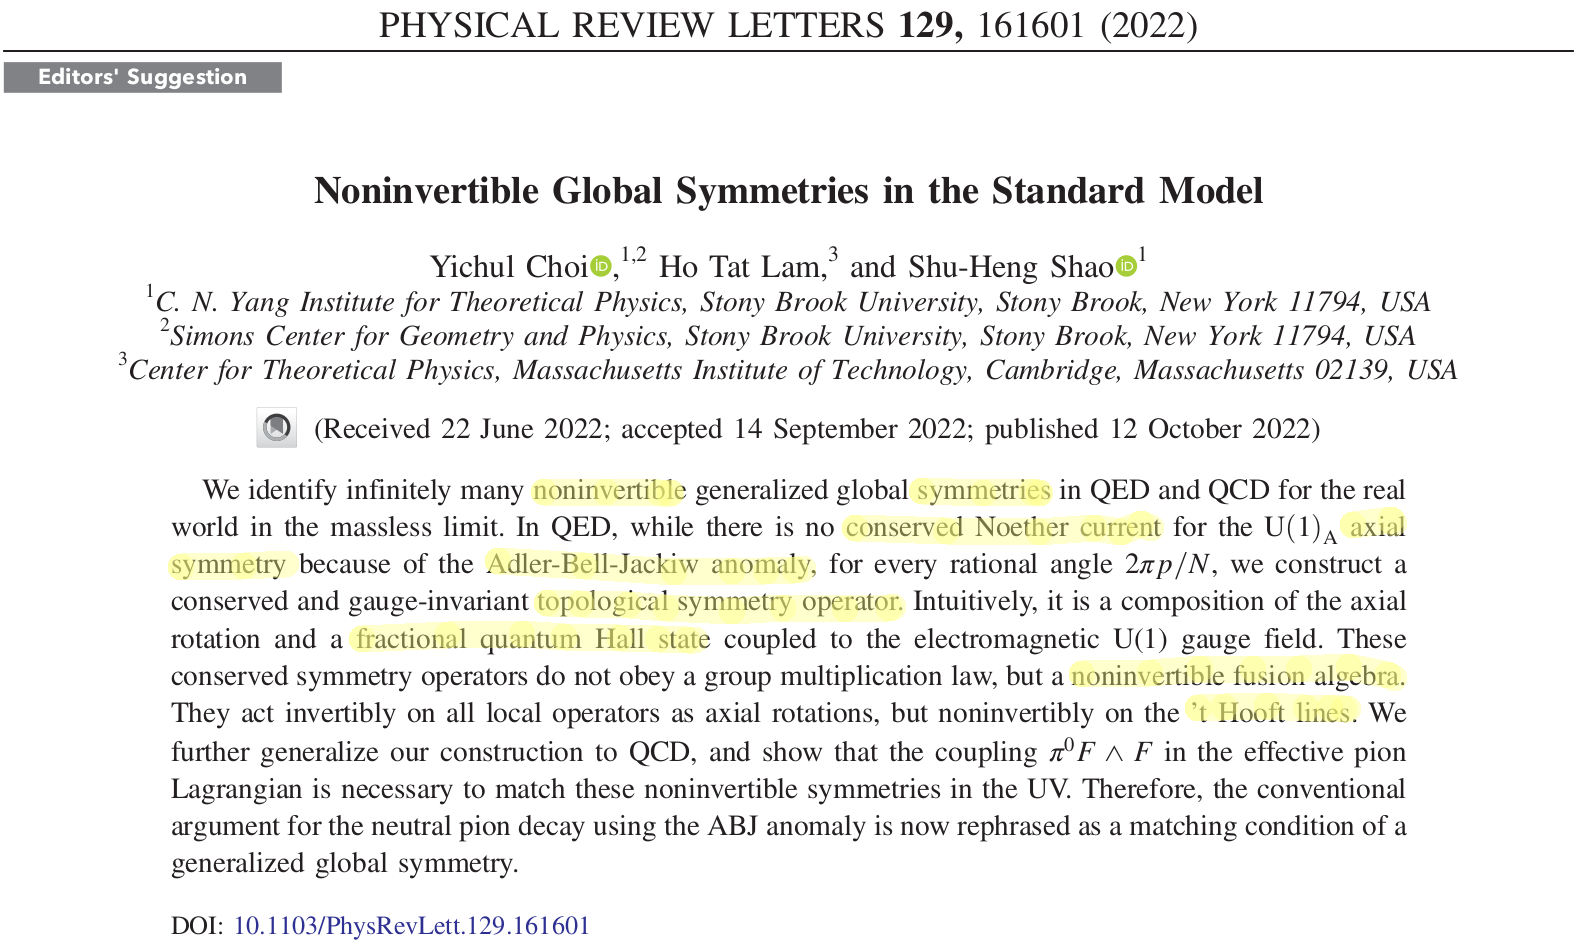
\includegraphics[scale=0.28]{abstract_interesting.png}
  \end{figure}
\end{frame}

\begin{frame}
  \frametitle{Symmetries?}
  \begin{itemize}
  \item Mathematically, symmetry $\Leftrightarrow$ group
  \item A \textbf{group} (of symmetries) represents \textit{a reasonable choice for what ``symmetry'' means in some context}.
  \item Symmetries are \textit{functions} that preserve a structure, in some sense.
  \item Groups are notations for these functions that decouple ``symmetry'' from ``thing that is symmetric''
  \end{itemize}
  \begin{figure}
    \begin{subfigure}{0.5\textwidth}
      \centering
      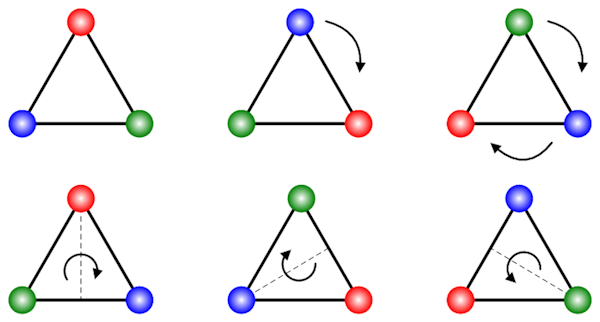
\includegraphics[width=0.8\linewidth]{tri-dihedral.png}
    \end{subfigure}%
    \begin{subfigure}{0.5\textwidth}
      \centering
      \begin{tikzcd}% [width=0.8\linewidth]
        S \arrow[loop right, "f"] \arrow[loop left, "g"] \arrow[loop above, "h"] \arrow[loop below, "1"]
      \end{tikzcd}
    \end{subfigure}
  \end{figure}
  A group is a set $G$ with a binary operation $\circ: G \times G \to G$ satisfying
  \begin{itemize}
  \item (Associativity) For all $f, g, h \in G$, $f \circ (g \circ h) = (f \circ g) \circ h = f \circ g \circ h$.
  \item (Identity) There exists $1 \in G$ satisfying $1 \circ a = a \circ 1 = a$.
  \item (\underline{Inverses}) For all $f \in G$, there's $f^{-1} \in G$ with $f \circ f^{-1} = f^{-1} \circ f = 1$.
  \end{itemize}
\end{frame}

\begin{frame}
  \frametitle{Symmetries?}
  To re-introduce the ``thing that is symmetric,'' there's the concept of an \textit{action},
  which produces the actual symmetry transformations:
  \begin{mydef}
    An \textbf{action} of a group $(G, \circ)$ on the set $A$ is a function $\circlearrowleft: G \times A \to A$ satisfying,
    for all $g, h \in G$ and $a \in A$,
    \begin{itemize}
    \item (Functor composition) $(g \circ h) \circlearrowleft a = g \circlearrowleft (h \circlearrowleft a)$;
    \item (Functor identity) $1 \circlearrowleft a = a$.
    \end{itemize}
  \end{mydef}

  Groups themselves can also have other structure; if there is \textit{smooth} structure,
  it is called a differentiable or Lie group.

  % Up to measure zero, everything's a matrix group.
  \[
    SO(3): \text{(axial) rotations, e.g. } \;
    \begin{pmatrix}
      \cos\phi & \sin\phi & 0 \\
      \sin\phi & \cos\phi & 0 \\
      0 & 0 & 1
    \end{pmatrix}
  \]
  \begin{center}
    flows along differential equations
  \end{center}
\end{frame}

\begin{frame}
  \frametitle{Gauge?}
  Often, arbitrary and nonphysical choices (made for computation's sake) produce ready-made symmetries.
  \begin{itemize}
  \item Choice of reference potential energy $\to$ ``change of zero'' transformation
  \item Choice of inertial frame $\to$ Poincar\'e (Lie) group
  \item Lagrangian mechanics doesn't change if $\mathcal{L}(t, q, \dot{q}) \mapsto \mathcal{L}(t, q, \dot{q}) + \grad{f}$
  \item The magnetic field doesn't change under $\vec{A} \mapsto \vec{A} + \curl{\vec{F}}$
  \end{itemize}

  Such are called \textbf{gauge symmetries} or \textbf{gauge groups}---the particular nonphysical choice being a \textbf{gauge}.

  \begin{itemize}
  \item QED $\to$ $U(1) = S^{1} \text{ with complex product}$
  \item QCD $\to$ $SU(3) = SO(3) \text{ but complex}$
  \end{itemize}
\end{frame}


\begin{frame}
  \frametitle{Conserved Noether Current?}
  Why are groups important in physics?
  \begin{thm}[Noether]
    If an (action) functional $S[q] = \int_{a}^{b}L(t, q, \dot{q})dx$ is invariant under the action of
    a one-dimensional Lie group $G$ on the base space,
    then a particular expression in terms of the integral kernel $L$ and quantities associated with $G$ must be constant.
  \end{thm}

  Invariant under $S[q(t)] \mapsto S[q(t + t_{0})]$ $\Leftrightarrow$ constant $\frac{1}{2}m\dot{q}^{2} + V(q)$

  This is why ``non-invertible symmetry'' makes sense in physics.
  If some structure isn't a group, but has a Noether-like theorem, then it's just as useful as a symmetry.
\end{frame}


\begin{frame}
  \frametitle{Non-Invertible Symmetry? Topological Symmetry?}
  In quantum mechanics, there's a \textbf{spin-statistics theorem}: multiparticle states are either fermionic or bosonic.
  \begin{itemize}
  \item Particle interchange: idempotent, linear operator on quantum states (a possible symmetry!).
  \item Bosons: $+1$ eigenstates of particle interchange.
  \item Fermions: $-1$ eigenstate of particle interchange.
  \item \textit{Proof requires dimension $> 2$!!}
  \end{itemize}

  The proof is Lie groups: $d > 2 \Rightarrow \pi_{1}(SO(d, 1)) \cong \pi_{1}(Po(d, 1)) \cong \mathbb{Z}_{2}$.
  \newline
  \begin{itemize}
  \item $d = 2 \Rightarrow \mathbb{Z}!$
  \item \textit{Infinitely many} possible statistics in two-dimensional systems!
  \item Called ``anyon'' quasiparticles.
  \end{itemize}

  Called ``topological'' behavior because $\pi_{1}$ is a \textbf{topological property}.
\end{frame}

\begin{frame}
  \frametitle{Non-Invertible Symmetry? Topological Symmetry?}
  Difference is intuitively understood via obstructions and knot theory.
  \begin{enumerate}
  \item 3D rotational symmetry lets one ``un-braid'' a particle interchange.
  \item Not so in 2D---confined to planar movements.
  \end{enumerate}
  \begin{center}
    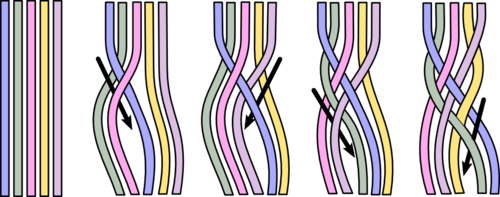
\includegraphics[scale=1.2]{braid.png}
  \end{center}
  These are non-invertible symmetries!
  Swapping particles and then swapping them back braids worldlines twice, instead of undoing it (monoid structure).
  There's nevertheless a conserved quantity associated with this symmetry (context: $n$-groups)---which makes it useful.
\end{frame}

\begin{frame}
  \frametitle{Fractional Quantum Hall Effect}
  Ordinary quantum and condensed-matter: quantum Hall effect.
  \begin{enumerate}
  \item Drude/Sommerfeld theory (kinetic theory + EM): current gets diagonal when magnetic field applied.
  \item Quantizes at high-$B$, low-$T$---$R_{H} = \frac{V_{H}}{I_{C}} = \frac{h}{e\nu}$
  \item Expected when $\nu = 1, 2, 3,\ldots$ but observed for $\nu = \frac{1}{3}, \frac{2}{5}, \frac{3}{7}, \ldots$!
  \end{enumerate}
  \begin{figure}
    \begin{subfigure}{0.5\textwidth}
      \centering
      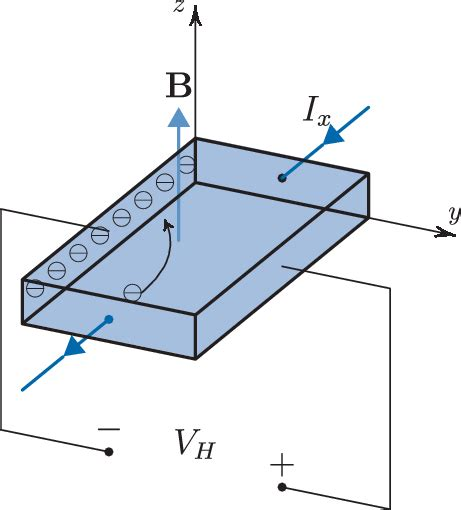
\includegraphics[width=0.6\linewidth]{he-app.png}
    \end{subfigure}%
    \begin{subfigure}{0.5\textwidth}
      \centering
      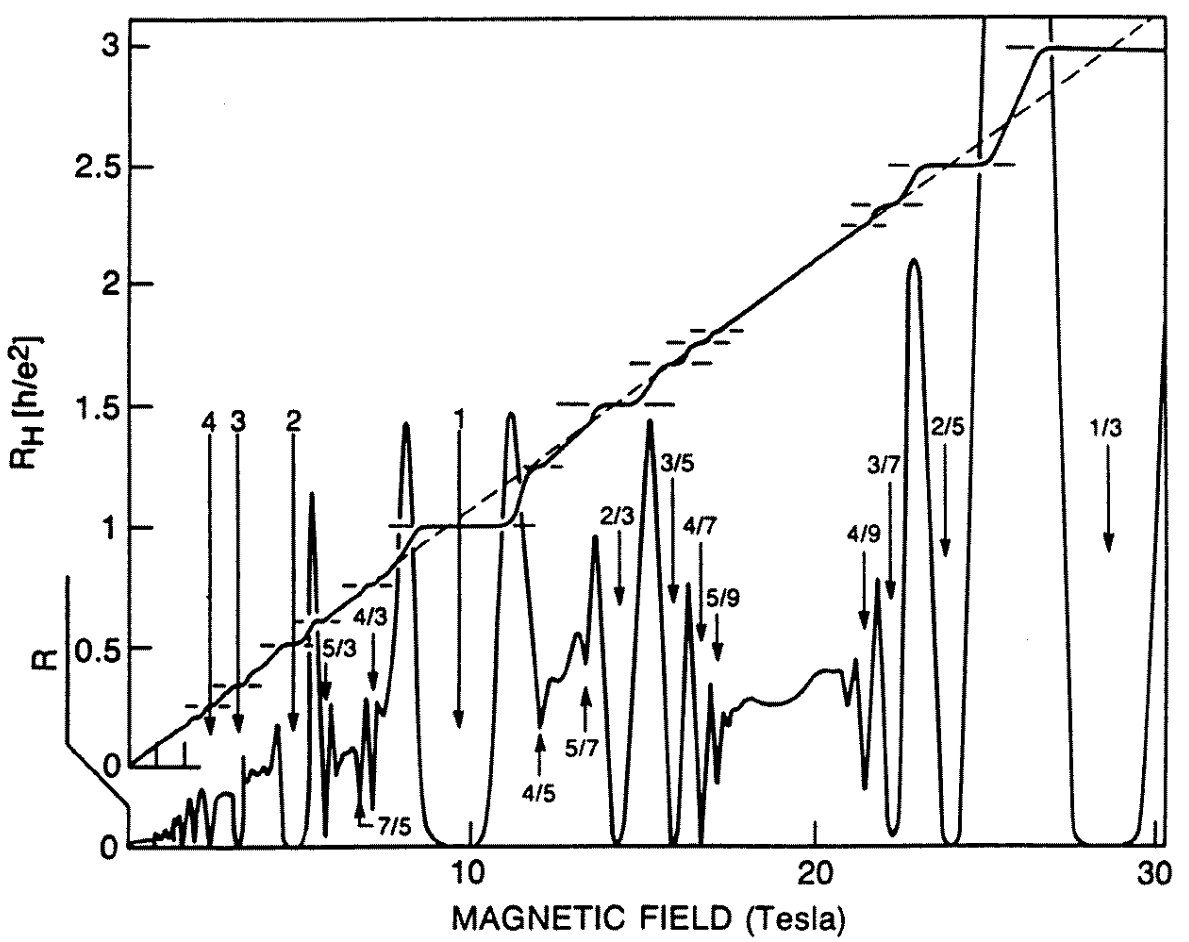
\includegraphics[scale=0.17]{fqhe.png}
    \end{subfigure}
  \end{figure}
  Now understood as quasiparticles with anyonic statistics---so there's a non-invertible symmetry operator!
\end{frame}

\begin{frame}
  \frametitle{ABJ Anomaly? $\pi^{0}$ Decay?}

  \begin{itemize}
  \item (Johnny) Classical $\to$ quantum $\Leftrightarrow$ $[A, B] = 0 \to [A, B] = i\hbar$.
  \item Sometimes, quantization breaks a symmetry: \textbf{Adler-Bell-Jackiw (ABJ, or chiral) anomaly}.
  \item This happens for QED with $U(1)$ (adding a phase $e^{i\phi}$); explains several CP-violating observations.
  \item Wrong width predicted for $\pi^{0} \to 2\gamma$ otherwise.
  \item (Predicts exactly 3 generations of quarks)
  \end{itemize}
  This paper: Standard Model conserves $U(1)$ composed with fractional quantum Hall operator,
  a gauge-invariant, non-invertible transformation with a corresponding conserved quantity.
\end{frame}

\begin{frame}
  \frametitle{Implications}

  \begin{itemize}
  \item For the first time: $\pi^{0}$ decay is necessary to \textit{preserve} a symmetry, rather than to explain \textit{breaking}.
  \item Borrows ideas from TQFT---an area of active \textit{mathematical} research (Joyal-Lurie $(\infty, 1)$-categories, HoTT).
  \item More symmetries = more ways to solve problems via symmetry arguments (think Gauss's law).
  \item New exactly-solvable QED/QCD systems?
  \item New mathematical structure of physical theories? (open question: what's the ``fusion algebra'' of these symmetries?)
  \item Application to axion theories?
  \item Other still-unknown symmetries?
  \end{itemize}
\end{frame}

\begin{frame}
  \frametitle{Appendix}

  \begin{figure}
    \begin{subfigure}{0.5\textwidth}
      \centering
      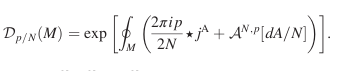
\includegraphics[width=\linewidth]{operator.png}
    \end{subfigure}%
    \begin{subfigure}{0.5\textwidth}
      \centering
      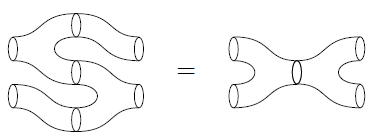
\includegraphics[scale=0.5]{tqft.png}
    \end{subfigure}
  \end{figure}
\end{frame}

\end{document}
%%% Local Variables:
%%% mode: latex
%%% TeX-master: t
%%% End:
